
\subsection{模态分析简介}
模态分析的主要问题是解广义特征值问题$|\mathbf{K}-\lambda\mathbf{M}|=0$的前几阶特征值及其对应的特征向量,因此我们把模态分析分为两个部分来进行:组装对应的刚度矩阵和质量矩阵,以及求解广义特征值问题.当我们把自由度选在节点上时,刚度阵就是静态分析中的刚度矩阵,因此我们只需要对于每个单元以类似的方法组装质量矩阵.对于求解广义特征值问题,我们使用的是子空间迭代法.
\subsection{程序实现}
在组装质量矩阵时,程序仅给出了杆单元的质量矩阵为例.对单元增加私有变量密度rho,并改变其读写函数,并增加纯虚函数组装质量矩阵ElementMass.我们使用的是一致质量矩阵,有$\mathbf{M}=\int\rho\mathbf{N}^T\mathbf{N}\mathrm{d}\Omega$,因此对于杆单元应当有

\[
\mathbf{M}=\frac{W}{3}\left(\begin{array}{cc} 2&1\\1&2 \end{array} \right)
\]

考虑到我们的杆单元是三维空间中的单元,因此对于左右还需进行坐标变换.

对广义特征值问题,首先给出初始向量$\mathbf{X}_1$以及$\mathbf{Y}_1=\mathbf{M}\mathbf{X}_1$,之后进入循环.在求得的特征值尚未收敛时,利用逆迭代法求下一步的$\mathbf{X}_{n+1}=\mathbf{K}^{-1}\mathbf{Y}_n$,$\mathbf{Y}_{n+1}=\mathbf{M}\mathbf{X}_{n+1}$,并求缩并后的矩阵$\bar{\mathbf{K}}=\mathbf{X}_{n+1}^T\mathbf{K}\mathbf{X}_{n+1}=\mathbf{X}_{n+1}^T\mathbf{Y}_n$, $\bar{\mathbf{M}}=\mathbf{X}_{n+1}^T\mathbf{M}\mathbf{X}_{n+1}=\mathbf{X}_{n+1}^T\mathbf{Y}_{n+1}$.这一部分直接在C++中编写代码运行,主要原因是考虑到将原矩阵扩充为对角阵或者带宽阵均会导致占用不必要的空间,我们小组有LDLT以及Pardiso两种求解器,目前振动模块只兼容LDLT,但将这一部分单独写出也方便之后改用稀疏求解器.

缩并后的矩阵由于维数一般不高,可以取上三角阵存储,方便后续输入LAPACK的对应求解驱动进行求解,这里我们使用的是LAPACKE\_dspgvd函数,这个函数的作用是对解三角存储的对称矩阵的广义特征值问题的所有特征值和特征向量.解得对应的特征值和特征向量之后,再利用选取的基向量把缩减自由度后的特征向量恢复至原坐标系中.如果特征值已经趋于收敛,那么跳出循环,得到的就是子空间迭代法的前n 阶特征值与特征向量.

\subsection{算例验证}
对于该模态分析的验证我们选取了一个一维的质弹系统,如图:

\begin{figure}[htbp]
  \centering
  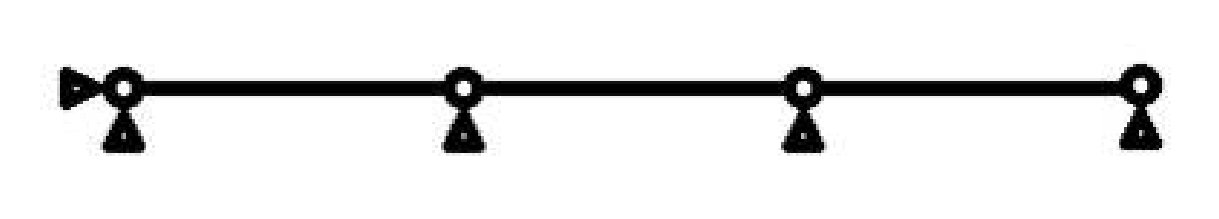
\includegraphics[height=1cm]{modalex}
  \caption{验证算例}
\end{figure}

取线密度为$1$,杨氏模量为$4\times 10^{10}$,横截面积为$1\times 10^{-2}$,每个杆长度为$1$.这样得到三个特征值与对应的特征向量分别为

\[
\lambda_1=1.219\times10^8,\lambda_2=1.2\times10^9,\lambda_3=3.9494\times10^9 \]

\[
\mathbf(d)_1=\left( \begin{array}{c} 0.3536 \\ 0.6124 \\ 0.7071 \end{array} \right),
\mathbf{d}_2=\left( \begin{array}{c} -0.7071 \\ 0.0000 \\ 0.7071 \end{array} \right),
\mathbf{d}_3=\left( \begin{array}{c} -0.3536 \\ 0.6124 \\ -0.7071 \end{array} \right) \]

当我们输入的要求特征值数为3时,得到的结果是准确的.当要求特征值数为2时,我们得到如下结果:

\[
\lambda_1=1.2196\times10^8,\lambda_2=1.24072\times10^9 \]

\[
\mathbf(d)_1=\left( \begin{array}{c} -0.4174 \\ -0.7248 \\ -0.8332 \end{array} \right),
\mathbf{d}_2=\left( \begin{array}{c} 1.0732 \\ -0.1402 \\ -0.8312 \end{array} \right) \]

考虑到特征向量没有进行正则化,可以发现一阶特征值以及特征向量误差极小,特征值的误差不超过千分之一,特征向量的误差在千分之四以下.而二阶特征值的误差则相对较大,特征向量的问题则更加显著.这些问题都是因为里兹基向量导致的,在原程序中我们没有使用特别的处理,仅通过逆迭代法逐渐放大对应阶数,因此容易出现这样的问题.在实际情况下,一般要求取前$n$阶特征值时,我们选取$\min (2n,n+8)$作为初始求取的特征值数.

\subsection{程序使用以及部分增加函数说明}
目前要通过程序计算振动模态,需要进行如下操作:在Cmake时增加勾选\_VIB\_的选项,并同时勾选\_DEBUG\_,这是因为不明链接原因导致二者必须同时勾选;同时不能使用USE\_MKL,因为虽然在程序中使用了MKL库,但是没用使用Pardiso求解器,因此会出现错误.之后还要打开Visual Studio之后手动打开MKL库,程序就能正常运行.

对于输入文件也要进行改动.对杆单元连接的质弹系统,在输入杆的材料时,材料参数增加为三个,输入顺序改为密度$\rho$,杨氏模量$E$,横截面积$A$.此外在输入所有单元之后,要继续输入要求解的特征值数.

程序中主要增加了函数bool CDomain::VibSolver(unsigned int NVibModes),输入参数为求解的特征值阶数.代码首先生成一个初始基向量组,这个初始基向量组可能不够好但是会随着逆迭代逐渐变好.在这里用到了我们定义的函数void CLDLTSolver::Multiple(double* acc, double* Force, unsigned int numeq, unsigned int vib\_m),用途是计算LDLT矩阵与列向量相乘的结果.下面定义循环中需要使用的动态数组并进入循环,循环中的内容如上程序实现介绍,最终释放动态数组.此外,程序中的assembly\_mass 与 AssembleMassMatrix等函数与对应的刚度矩阵函数的意义是相似的,只不过是改为组装质量矩阵.

